\section{Prestudy}
\label{sec:prestudy}
%Intro - what the prestudy was
In order to inform the development of the project, and provide a reasonable basis for some of the design decisions made about the system, an initial prestudy was run with questions covering a wide range of relevant areas.
%Justifications - some detail about contents
The primary intention of the survey was to find out how people currently consume TV programmes and related streaming media, and their responses to the adverts that support the services they use.
There were questions on format and frequency of media consumption, and typical actions during advertisement presentation.
The study also included questions about individual levels of acceptance of the use of personal information for advertisement targeting, and an opportunity to share further personal opinions and comments in an optional free text question.
%Conclusion - the prestudy was useful
Ultimately, the wide coverage of questions gave many useful insights into existing viewer habits and responses.

%Intro - what the data was for
The main use of the data collected during the survey was to support and justify system development decisions throughout the course of the project. 
%Justification - specific hopes for the results
The questions were written to elicit information from the participants in support of several specific purposes, in addition to the basic background information about existing viewing habits.
One intended function of the results was to establish which features of an advert had the most influence on user attention -- this would allow development to be focused upon the best techniques to retain user attention to adverts, thereby making the product a more desirable option for advertisers, and resulting in greater profits for advertisers and greater satisfaction for users.
Another intended outcome was to discover whether typical advertisement responses provided scope for alternative attention retention techniques; for example, if users typically refocused their activities onto other devices during advertisement breaks, the provision of audio-only advertisements could provide an avenue for successful impressions despite loss of visual attention.
%Conclusion - the data was relevant
Determining how users respond to existing adverts in existing systems was an important prerequisite to tailoring development work so that the system is as effective as possible, and the survey questions were designed to support that aim.


% Purpose of the study:\\
% Collect data on how people consume media and adverts\\
% Inform the development of features for the project\\
% Elicit basic information about viewer habits

\subsection{Methodology}

% The prestudy was performed early in the project --- 10/20/2012 --- to allow the results to be considered into the design of your4.tv. The study was hosted as a short questionnaire online at the url \url{www.http://your4.tv/#prestudy}, designed to be easy and quick to fill out to maximise responses, with each entry automatically entered into a spreadsheet upon submission. At the time of writing, the prestudy is still available online, and a listing of the prestudy questions can be found in Appendix~\ref{sec:appendix_prestudy_questions}.

% The url was shared amongst a demographic of students, the target audience of the system, where each submission was anonymous, and run for 7 days gathering 67 responses before the results were analysed.

% The prestudy page as presented to participants is available at \href{http://your4.tv/\#prestudy}{\texttt{your4.tv/\#prestudy}} 

%Intro - we wanted efficiency
To help ensure that the prestudy results were relevant and informative, close attention was paid to certain aspects of the study methodology.
%Justification - this was how we got it
%-Selected students as a sample - representative (find reference)\\
\citet{viacom} reports that young people (the 18-24 demographic) watch TV on tablets more than any other demographic, and so the prestudy was directed largely towards this group. %TODO Maybe mention Project4's target audience, and available adverts
%-Protected results, ethics number 4315\\
Following the guidelines of the governing body, the questionnaire draft was submitted to ERGO, and recieved ecthical approval to proceed (study number 4315). %TODO - mention password protected and automatic
%-Performed early\\
Since the survey outcomes were an important influencing factor in the continued development of the system, it was essential that the prestudy was completed early in the lifetime of the project. Once the intention and form of the questions had been finalised, the survey was created and publicised as swiftly as possible.
%Conclusion - aspects of how the survey was run made it more successful
By releasing the study quickly and advertising it specifically to the target demographic, maximal value was derived from the outcomes. %TODO: gah.

%Intro - we wanted lots of data
So that anomalous results did not unduly skew the outcome of the study, and to ensure broad coverage and increase the possible diversity of viewpoints captured, it was important to attempt to maximise the number of responses the survey would recieve.
%Justification - we did these things to induce people to answer
%We were also keen to ensure that as many people as possible would provide useful information
%-Short and easy and anonymous\\
One approach taken was to make the questionnaire as quick and painless as possible to complete.
The survey design was intentionally short and minimal, with the majority of the questions answerable via checkboxes or radio-buttons.
No personally identifiable information was collected, and the only question requiring a full text answer was optional. %TODO: talk about using an URL %(who wrote this?)
%-Webpage\\
A web-based service was used to host the survey, which helped to ensure participant anonymity and data security, ease of access to the survey itself, and also automatic answer collation and streamlined processing.
%-Spread via social networking sites\\
Finally, the survey itself was largely advertised via social networking sites. Aside from the benefits of serendipitous discovery, this also helped to ensure that potential participants were most likely to find the survey during times when they would also have opportunity to quickly complete it.
%Conclusion - This helped: we got a large number of results as discussed in the following section
Initially the prestudy completion target was set at 30 respondants, however due in at least some part to the techniques employed during its design, the final count was more than double this figure -- as discussed in the following section. %TODO: is this too wooly?


%Note
The prestudy page as presented to participants is still available online\footnote{Your4 Prestudy Questionnaire -- \footurl{http://your4.tv/\#prestudy}}, and a listing of the questions can be found in Appendix~\ref{sec:appendix_prestudy_questions}. 


\subsection{Outcomes}

%Stats
%Intro - the survey was in some respects more successful than hoped
In many respects the survey was more successful than anticipated.
%Justification
%-Over the course of a single week
Over the course of a single week, the online survey was seen and completed by a large number of participants.
%-67 student participants
In total, 67 responses were recorded, covering a wide variety of viewpoints and supplying several useful datapoints about viewer habits and responses.
%-Discovered specific features we should focus on
These led to a number of specific features that were selected for further attention - and a number that were disregarded.
%Conclusion - this was a good thing
In terms of depth and breadth of feedback recieved, the prestudy provided a sound, results-backed basis for many of the development decisions throughout the project.

%Specific outcomes
%INtro - there are some specific things we can pick up on
Some of the data recorded during the prestudy was particularly relevant to the system specification process, while other questions produced responses that were more useful for informing a fuller picture of the context and demographic backround.
%Justification
%Bacground - section .1
For example, the first few questions were intended to give a clearer view of how often respondants watched streaming media in various formats, and how the attention paid to adverts varied by format -- revealing that most attention was given to adverts shown on live TV (see section~\ref{sec:prestudy_media}).
%Relevant adverts - section .2
Other data revealed which specific aspects of an advert were likely to have an influence on whether it was watched by a viewer, as discussed in section~\ref{sec:prestudy_influence}.
%Ability to skip adverts - section .3
When considering adverts that were not watched by viewers, it was also useful to discover what actions were typically taken instead (section~\ref{sec:prestudy_alternatives}), in order to investigate alternative methods through which overall advert impressions could be reasonably maximised.
%Targeting
Additionallly, the prestudy questions anticipated a likely direction for the project and investigated acceptence of the use of personal information to improve advertisement relevance, revealing that most of the respondants were comfortable with some degree of targeting.
%Conclusion - IN this light, suggests that the product we propose will improve the ...
The survey results suggest that the proposed product will most easily be able to improve upon existing offerings by providing a TV-like experience with specific additional functionality, rather than trying to pursue an experience more akin to that supplied by traditional in-browser video sources.

%Interesting free text responses
%Intro - of particular note:
%Justification - find some of these
%Conclusion - variety of viewpoints out there



A detailed breakdown of some specific questions follows

\subsubsection{Attention by media type}
\label{sec:prestudy_media}
%Question: How often do you pay attention to adverts served with the following media?
\begin{figure}[H]
	\vspace{-10pt}
	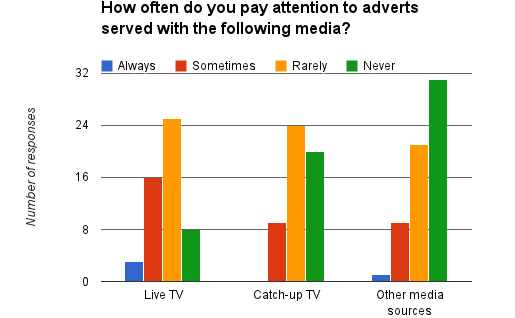
\includegraphics[width=\textwidth, clip=true, trim=0 0 0 50pt]{images/prestudy_media.png}
	\caption{User responses to the question ``How often do you pay attention to adverts served with the following media?''}
	\label{fig:prestudy_media}
	\vspace{-15pt}
\end{figure}
As can be seen in Figure~\ref{fig:prestudy_media}, only a small minority of participants reported to always pay attention adverts shown. In particular, amongst viewers watching other media such as Youtube, more than half of them never watch any of the advertisements at all - from the free text responses, it seem this is largely people using ad blocking programs. On the other hand, a far larger proportion of viewers `Always' or `Sometimes' watch adverts on live TV, which is certainly good news for a platform such as your4.tv.

\subsubsection{Influential Aspects}
\label{sec:prestudy_influence}
%Question: How much do the following aspects influence how likely you are to watch an advert?
\begin{figure}[H]
	\vspace{-10pt}
	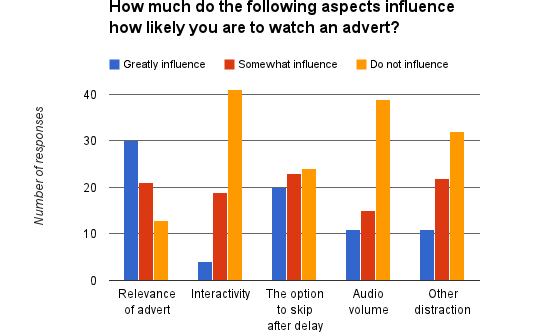
\includegraphics[width=\textwidth, clip=true, trim=0 0 0 50pt]{images/prestudy_influence.png}
	\caption{User responses to the question ``How much do the following aspects influence how likely you are to watch an advert?''}
	\label{fig:prestudy_influence}
	\vspace{-15pt}
\end{figure}
Finally, we looked at which specific aspects affected why people were likely to watch an advert (or not), with some interesting results. The two factors with the largest influence were the relevance of the advertisement and whether or not there was opportunity to skip it - both of which are addressed in the service we are developing. We also found, through analysing the free text responses, that people have a generally poor opinion of adverts that force a response from the user, whether they be obnoxiously loud, or simply require the user to interact with them before delivering content. Again, we can refer to these findings to help us to design a product that people will actually use. 
%TODO: do we mention the retrospecive need to define positive vs. negative influence?



\subsubsection{Advertisement responses}
\label{sec:prestudy_alternatives}
%Question: If you do not pay attention to adverts, which of the following do you do instead? (multiple choice)
\begin{figure}[H]
	\vspace{-10pt}
	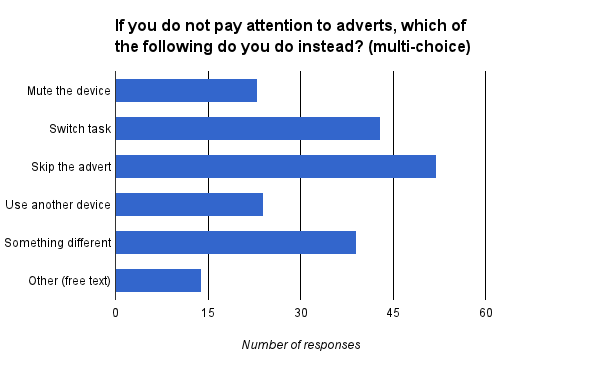
\includegraphics[width=\textwidth, clip=true, trim=0 0 0 50pt]{images/prestudy_alternatives.png}
	\caption{User responses to the question ``If you do not pay attention to adverts, which of the following do you do instead?''}
	\label{fig:prestudy_alternatives}
	\vspace{-15pt}
\end{figure}
Having seen that almost everyone ignores adverts sometimes, we also asked what people did instead of paying attention to them. Again, we can see that more than three quarters of the respondents skip adverts at least occasionally, where possible. We found that a few of the respondents mentioned `zoning out' and losing interest during ad breaks - we can also see that people use the advertisement time to do other tasks - generally on the same device, but less frequently on another one, or something completely different like making tea, etc. We use this data to help inform the development of functionality for the system.
